\section{Contraintes}

\subsection{Charge de travail}
La charge de travail est directement liée à plusieurs critères : le temps,
l'effectif disponible et les compétences de chacun des membres. L'équipe COGITO que nous 
composons et qui a réalisé ce projet est composée de
quatre étudiants en Master informatique première année (DECOL\footnote{Master
DECOL : Données Connaissances et Langage Naturel.} et IMAGINA\footnote{Master
IMAGINA : Images, Games and Intelligent Agents.}). Certaines compétences 
nécessaires à la réalisation de ce travail n'étaient pas
acquises lors du démarrage du projet, ce qui demande un temps d'adaptation
supplémentaire. Le projet s'est déroulé du mois de Février au mois d'Avril, soit environ trois
mois de réalisation, période durant laquelle devaient être effectuées les tâches
suivantes :

\begin{itemize}
\item étude du sujet, 
\item formalisation, 
\item développement, 
\item évaluation,
\item et préparation du rendu (rédaction du présent rapport et préparation de la soutenance).
\end{itemize}

Nous avons donc dû effectuer un gros travail de simplification du modèle initial en restant modeste, afin de pouvoir offrir un outil aboutit et fonctionnel à la date du rendu.

\section{Restrictions}

\subsection{Aperçu général des limitations appliquées}

La figure~\ref{modele_restreint} met en évidence le sous ensemble que nous avons choisi d'étudier, qui a été déterminé à partir des contraintes énumérées au chapitre~\ref{chapter:les_contraintes}. Cette sous partie correspond à ce que Laborit nomme le néocortex.

\begin{figure}[H] 
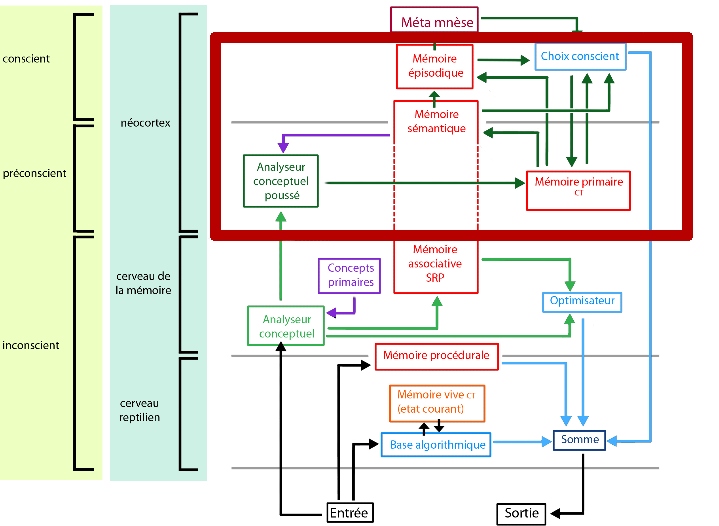
\includegraphics[width=\textwidth]{files/modele_restreint} 
\caption{Modèle restreint déterminé à partir des contraintes énumérée au chapitre~\ref{chapter:les_contraintes}} 
\label{modele_restreint}
\end{figure}

\subsection{Domaine d'application : le jeu de plateau}
\label{section:domaine_application_le_jeu_de_plateau}

%----------------------------------------
% DOMAINE D'APPLICATION : POUQUOI
%----------------------------------------
\begin{frame}{Domaine d'application}{Jeu de plateau}

\begin{block}{Pourquoi le jeu de plateau ?}
\begin{itemize}
\item Convergence \texttt{DECOL} / \texttt{IMAGINA}.
\pause
\item Activité purement cognitive.
\pause
\item Activité cognitive complète.
\pause
\item Évaluation facile de la performance.
\end{itemize}
\end{block}

\end{frame}


%----------------------------------------
% LE MINIMAX
%----------------------------------------
\begin{frame}{Domaine d'application}{Théorie des jeux}

\begin{block}{Théorème du MiniMax}
\begin{itemize}
\item J. Von Neumann, 1928.
\item \textit{Stratégie optimale pour un joueur donné.}
\end{itemize}
\end{block}
\end{frame}


%----------------------------------------
% LIMITES DU MINIMAX
%----------------------------------------

\begin{frame}{Domaine d'application}{Limites du MiniMax}

\begin{block}{Type de confrontation}
\begin{itemize}
\item \underline{Minimax}: Jeux compétitifs, à deux joueurs, à somme nulle.
\item \underline{Minimax \& Nash}: Durée et nombre d'options finis.
\end{itemize}
\end{block}

\pause

\begin{block}{Temps de calcul}
\begin{itemize}
\item En moyenne \emph{$O(b^{\frac{d}{2}})$} :
	\begin{itemize}
	\item d : longeur partie.
	\item b : options par tour.
	\end{itemize}
\item En pratique : besoin d'heuristiques $\Rightarrow$ perte d'optimalité.
\end{itemize}
\end{block}

\end{frame}